\documentclass[a4paper, 12pt]{article}

% Для многоязычности
\usepackage{polyglossia}
\setdefaultlanguage[indentfirst=true,spelling=modern]{russian}
\setotherlanguage{english}
% Юникодные математические символы
\usepackage{unicode-math}

\usepackage{amsmath}

\usepackage{fontspec}
% Подключаем шрифт. Шрифт есть в дистрибутиве TeXLive
\setmainfont[Ligatures={Common,TeX},Scale=0.94]{IBM Plex Serif}
\setromanfont[Ligatures={Common,TeX},Scale=0.94]{IBM Plex Serif}
\setsansfont[Ligatures={Common,TeX},Scale=MatchLowercase,Scale=0.94]{IBM Plex Sans}
\setmonofont[Scale=MatchLowercase,Scale=0.94,FakeStretch=0.9]{IBM Plex Mono}

% Математический шрифт
\setmathfont{STIX Two Math}

\usepackage{setspace}
\onehalfspacing

\usepackage[backend=biber,sorting=none]{biblatex}
\addbibresource{bib/cite.bib}

% Пакет для подключения картинок
\usepackage{graphicx}
% Пакет для ссылок (hyper references)
\usepackage[hidelinks]{hyperref}

\usepackage{listings}
\usepackage{xcolor}
\lstdefinestyle{mystyle}{
    backgroundcolor=\color{black!5},
    commentstyle=\color{green!40!black},
    keywordstyle=\color{magenta},
    stringstyle=\color{purple},
    basicstyle=\footnotesize\ttfamily,
    numbers=left,
    breaklines=true,
    numberstyle=\tiny\color{black!60},
    frame=tb,
    framerule=0pt,
}
\lstset{style=mystyle}

\usepackage{float}
\usepackage{lipsum} % Для генерации текста-"рыбы"


\renewcommand{\figurename}{Рис.}
\renewcommand{\tablename}{Таблица}
\renewcommand{\lstlistingname}{Листинг}
\renewcommand{\contentsname}{Содержание}
\renewcommand{\listfigurename}{Список иллюстраций}
\renewcommand{\listtablename}{Список таблиц}
\renewcommand{\lstlistlistingname}{Список листингов}

\usepackage{geometry}
\geometry{left=2.5cm, right=1.5cm, top=2cm, bottom=2cm}

\author{Николаев Дмитрий Иванович, НПМмд-02-24}
\title{Лабораторная работа №4: Включение графики и создание перекрестных ссылок в \LaTeX \\ Computer Skills for Scientific Writing}
\date{\today}

\begin{document}
  \maketitle
  \tableofcontents
  \pagebreak

  \listoffigures
  \lstlistoflistings
  \pagebreak

\section{Цель работы}
Целью данной работы является изучение и практическое освоение средств работы с графикой и перекрёстными ссылками в \LaTeX. 

\section{Теоретическое введение}
Визуализация данных и удобная навигация по документу являются неотъемлемыми атрибутами качественной научной работы. \LaTeX предоставляет достаточно гибкие инструменты для включения графических материалов (растровых и векторных изображений, диаграмм, графиков) и создания системы перекрёстных ссылок, которая автоматически обновляется при изменениях в документе.

Основным инструментом для вставки изображений является пакет \texttt{graphicx} с его командой \texttt{\textbackslash includegraphics}. Для управления расположением изображений используются "плавающие" окружения, такие как \texttt{figure}. Механизм ссылок строится на паре команд \texttt{\textbackslash label} (для создания "якоря") и \texttt{\textbackslash ref} (для ссылки на него). Пакет \texttt{hyperref} расширяет эту функциональность, превращая ссылки в кликабельные гиперссылки в итоговом PDF-документе.

\section{Выполнение лабораторной работы}
В процессе выполнения работы был создан файл \texttt{lab4.tex} (а также \texttt{lab4\_2column.tex} для одного задания), в который последовательно добавлялись примеры из пособия и решения упражнений.

\subsection{Часть 1: Последовательное воспроизведение примеров из пособия}

Будем выполнять задания из пособия~\cite{lab}.

\paragraph{1.1. Базовая вставка изображения.}
Для начала работы был подключен пакет \texttt{graphicx}. Изображение было вставлено с помощью команды \texttt{\textbackslash includegraphics} и отцентрировано с помощью окружения \texttt{center}. Код приведён в \lstlistingname~\ref{lst:part1_1}, результат на \figurename~\ref{fig:001}.

\begin{lstlisting}[
    float=htbp,
    language=tex,
    caption={Базовая вставка изображения},
    label=lst:part1_1
]
\documentclass{article}
\usepackage[T1]{fontenc}
\usepackage{graphicx}
\begin{document}
This picture
\begin{center}
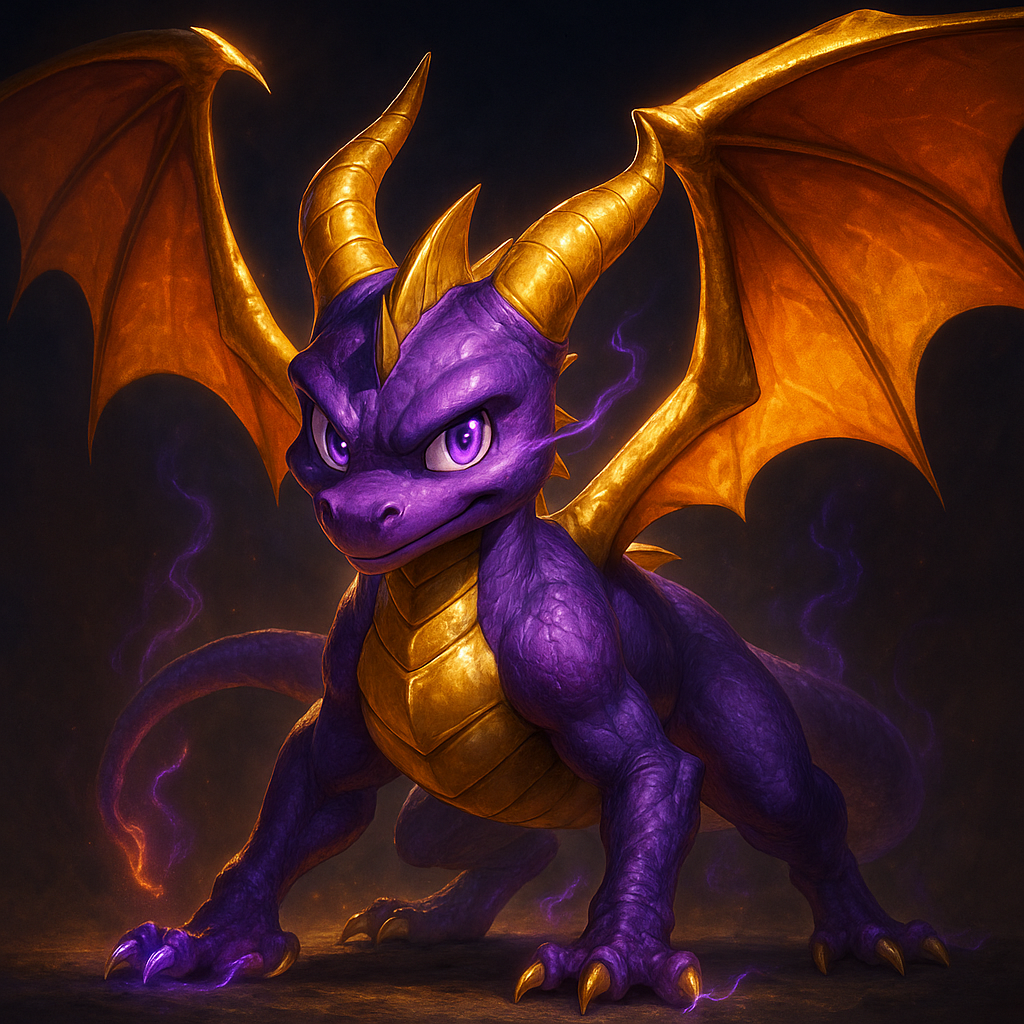
\includegraphics[height=2cm]{example-image.png}
\end{center}
is an imported PDF.
\end{document}
\end{lstlisting}

\begin{figure}[!htbp]
    \centering
    
\includegraphics[width=0.8\textwidth]{image/1.png}
    \caption{Результат базовой вставки изображения}
    \label{fig:001}
\end{figure}

\paragraph{1.2. Изменение внешнего вида графики.}
Были изучены опции для масштабирования изображения относительно высоты (\texttt{\textbackslash textheight}) и ширины (\texttt{\textbackslash textwidth}) текстового блока, а также опции для кадрирования (\texttt{trim}) и обрезки (\texttt{clip}). Код показан в \lstlistingname~\ref{lst:part1_2}, результат --- на \figurename~\ref{fig:002_1}--\ref{fig:002_2}.

\begin{lstlisting}[
    float=htbp,
    language=tex,
    caption={Масштабирование и кадрирование изображения},
    label=lst:part1_2
]
% --- Масштабирование ---
\begin{center}
    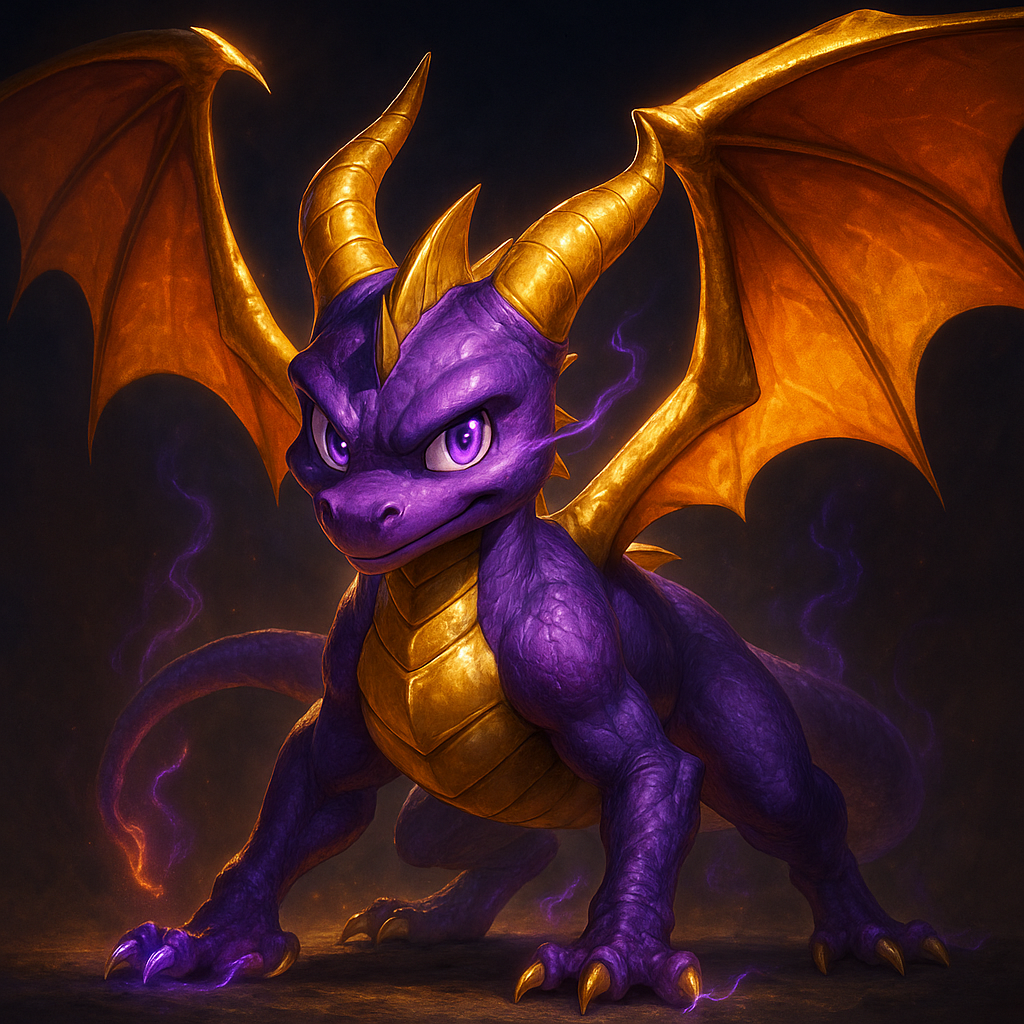
\includegraphics[height = 0.5\textheight]{example-image.png}
\end{center}
Some text
\begin{center}
    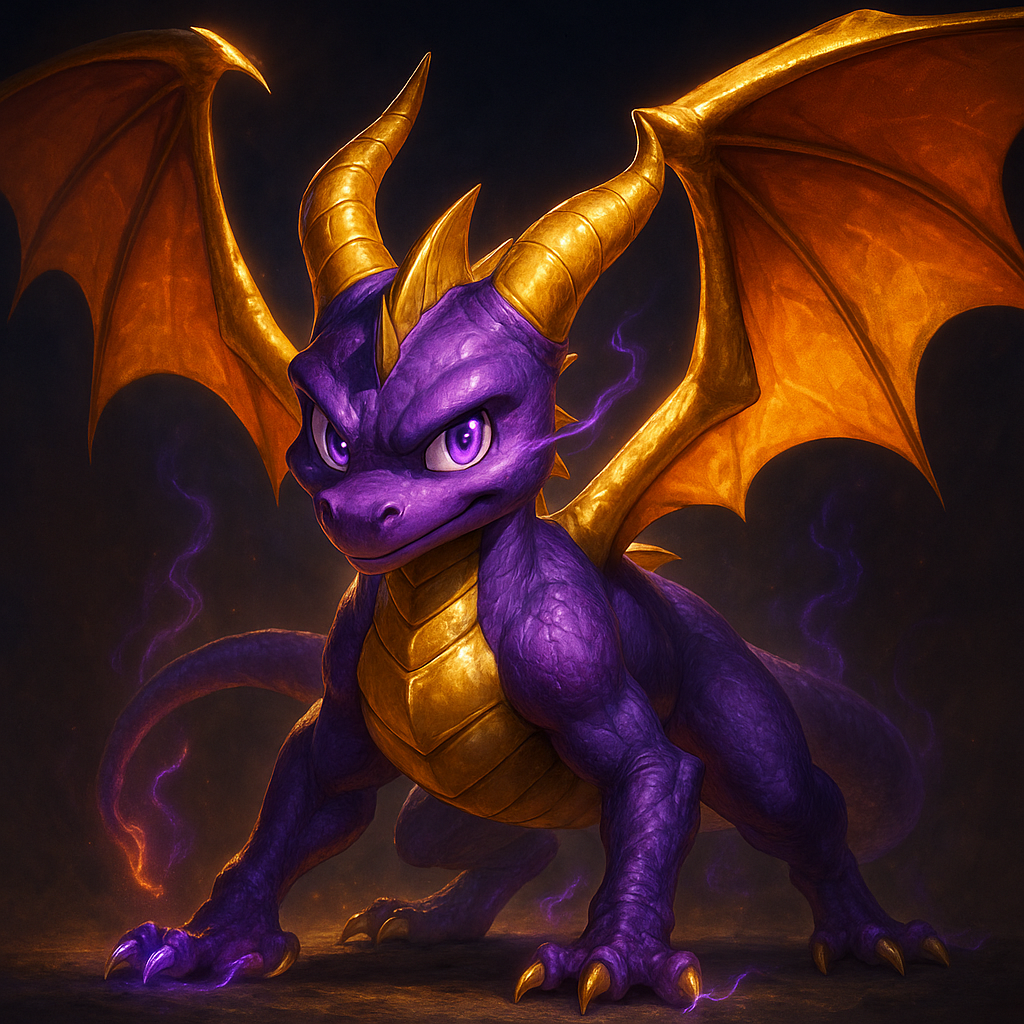
\includegraphics[width = 0.5\textwidth]{example-image.png}
\end{center}

% --- Кадрирование ---
\begin{center}
    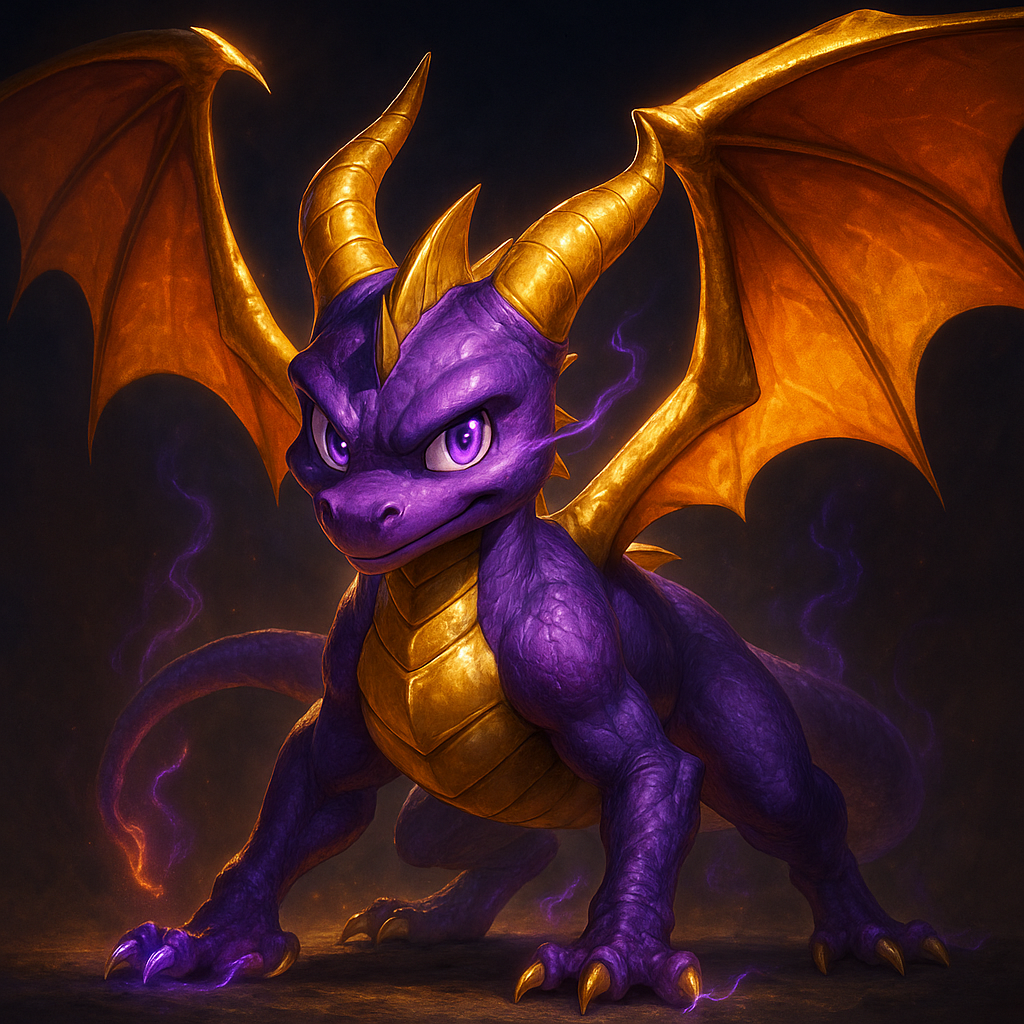
\includegraphics[clip, trim = 0 0 50 50]{example-image.png}
\end{center}
\end{lstlisting}

\begin{figure}[!htbp]
    \centering
    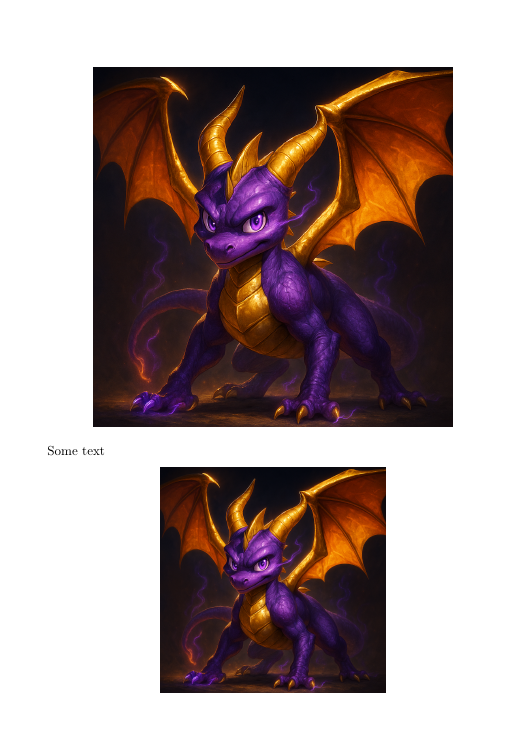
\includegraphics[width=0.8\textwidth]{image/2_1.png}
    \caption{Масштабированные изображения}
    \label{fig:002_1}
\end{figure}

\begin{figure}[!htbp]
    \centering
    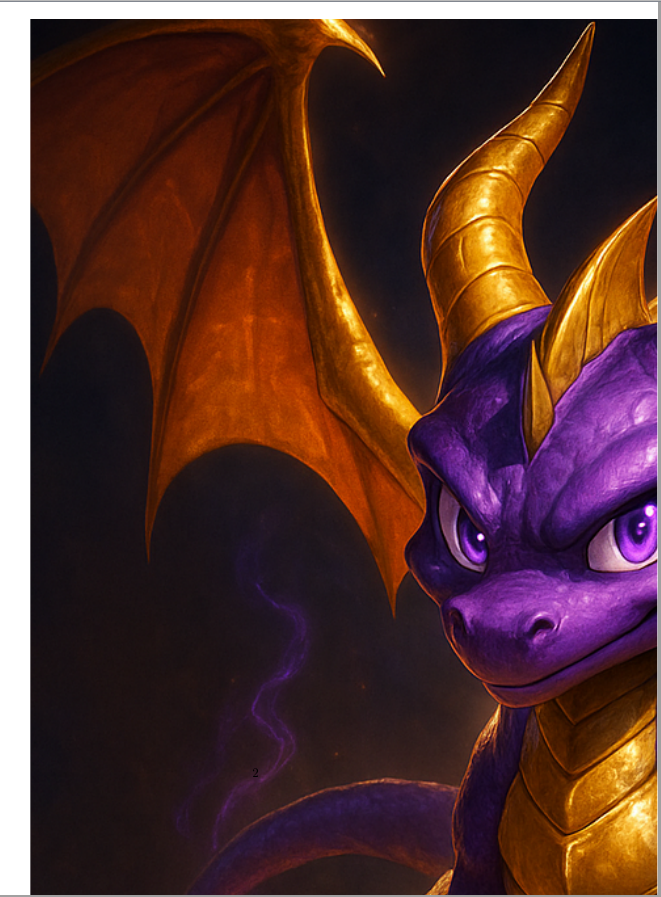
\includegraphics[width=0.8\textwidth]{image/2_2.png}
    \caption{Кадрированное изображение}
    \label{fig:002_2}
\end{figure}

\paragraph{1.3. Плавающие окружения.}
Для корректного обтекания рисунков текстом используется плавающее окружение \texttt{figure}. С помощью пакета \texttt{lipsum} был добавлен демонстрационный текст, показывающий, как \LaTeX автоматически перемещает рисунок в подходящее место (например, наверх следующей страницы, как в данном примере), чтобы избежать больших пустых пространств. Код приведён в \lstlistingname~\ref{lst:part1_3}, результат на \figurename~\ref{fig:003}.

\begin{lstlisting}[
    float=htbp,
    language=tex,
    caption={Использование плавающего окружения figure},
    label=lst:part1_3
]
\usepackage{lipsum} % produce dummy text as filler
...
\lipsum[1-4] % Just a few filler paragraphs
Test location.
\begin{figure}[ht]
    \centering
    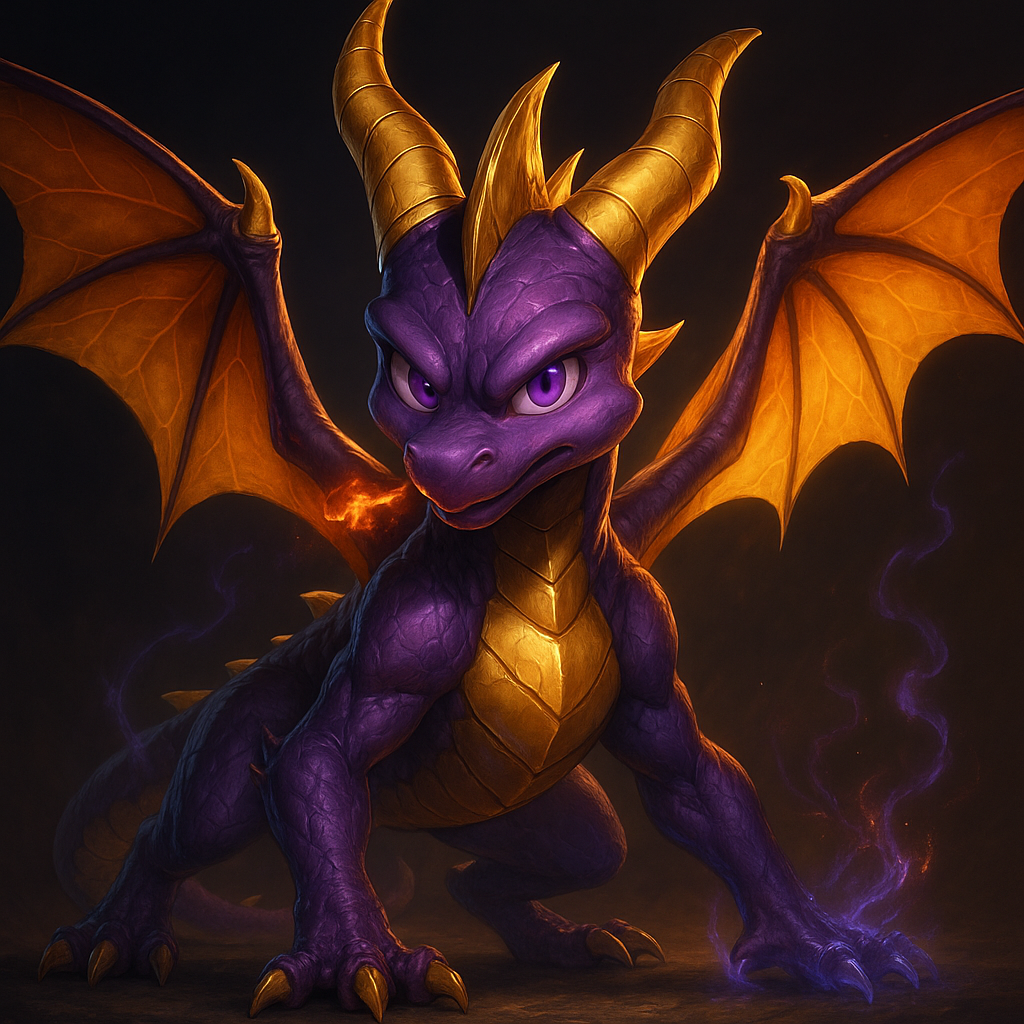
\includegraphics[width=0.5\textwidth]{example-image-a.png}
    \caption{An example image}
\end{figure}
\lipsum[6-10] % Just a few filler paragraphs
\end{lstlisting}

\begin{figure}[!htbp]
    \centering
    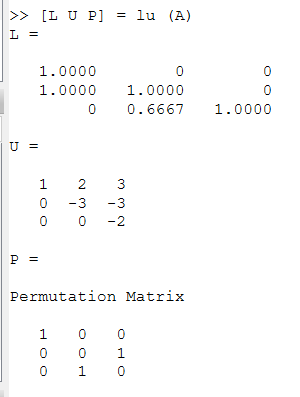
\includegraphics[width=0.8\textwidth]{image/3.png}
    \caption{Работа механизма плавающих окружений}
    \label{fig:003}
\end{figure}

\paragraph{1.4. Хранение графики в подкаталоге.}
Для лучшей организации проекта была использована папка \texttt{image}, в которую было помещено изображение. Команда \texttt{\textbackslash graphicspath\{\{image/\}\}} в преамбуле позволила \LaTeX автоматически искать файлы в этой папке. Код показан в \lstlistingname~\ref{lst:part1_4}, результат --- на \figurename~\ref{fig:004}.

\begin{lstlisting}[
    float=htbp,
    language=tex,
    caption={Использование \texttt{\textbackslash graphicspath}},
    label=lst:part1_4
]
% В преамбуле документа:
\graphicspath{{image/}}
...
% В теле документа:
An image from directory
\begin{figure}[ht]
\centering
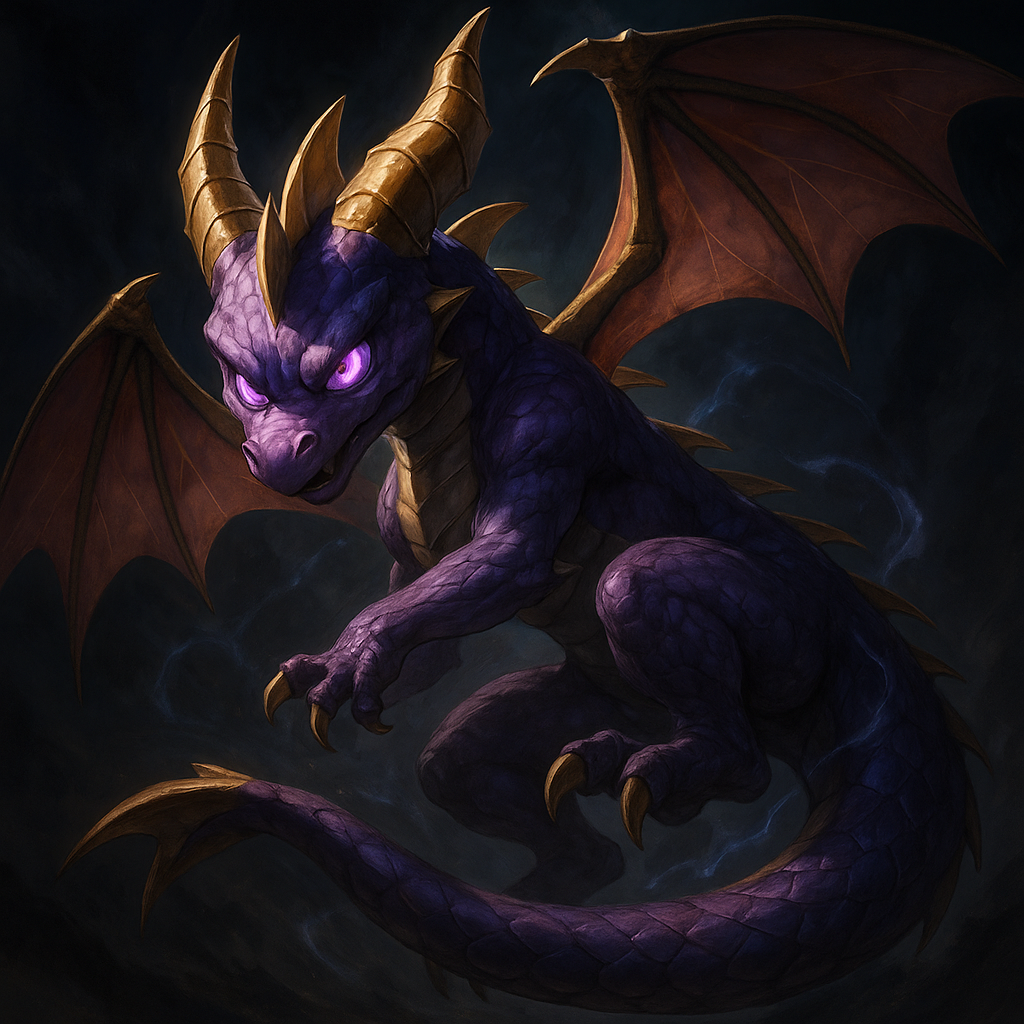
\includegraphics[width=0.5\textwidth]{example-image_b.png}
\caption{An example image from directory}
\end{figure}
\end{lstlisting}

\begin{figure}[!htbp]
    \centering
    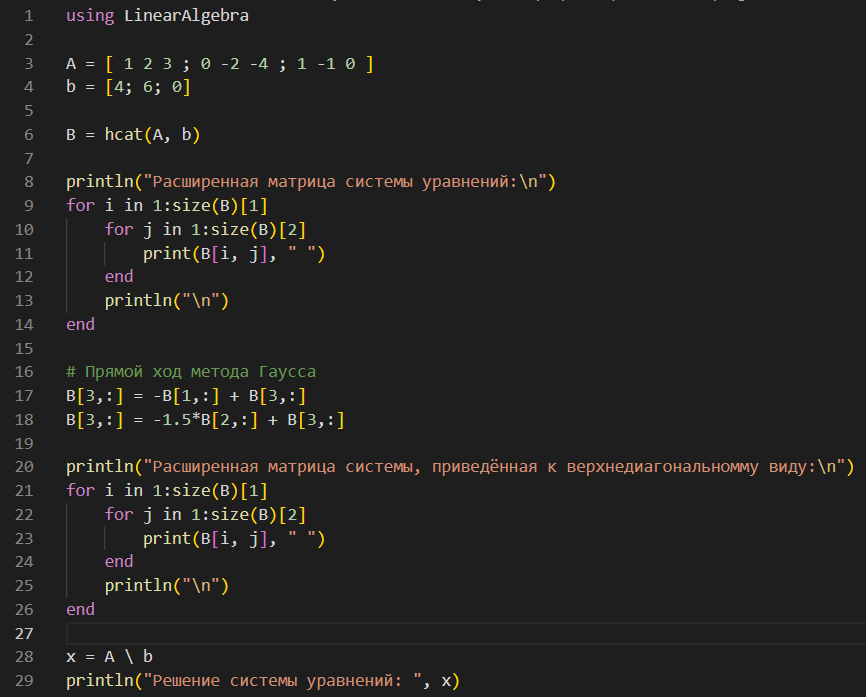
\includegraphics[width=0.8\textwidth]{image/4.png}
    \caption{Вставка изображения из подкаталога}
    \label{fig:004}
\end{figure}

\paragraph{1.5. "Жёсткая" фиксация положения.}
Иногда требуется запретить \LaTeX'у перемещать изображение. Для этого используется пакет \texttt{float} и опция \texttt{[H]} (Here) у окружения \texttt{figure}. Код представлен в \lstlistingname~\ref{lst:part1_5}, результат --- на \figurename~\ref{fig:005}.

\begin{lstlisting}[
    float=htbp,
    language=tex,
    caption={"Жёсткая" фиксация с пакетом float},
    label=lst:part1_5
]
\usepackage{float}
...
\lipsum[1-8]
\begin{figure}[H]
\centering
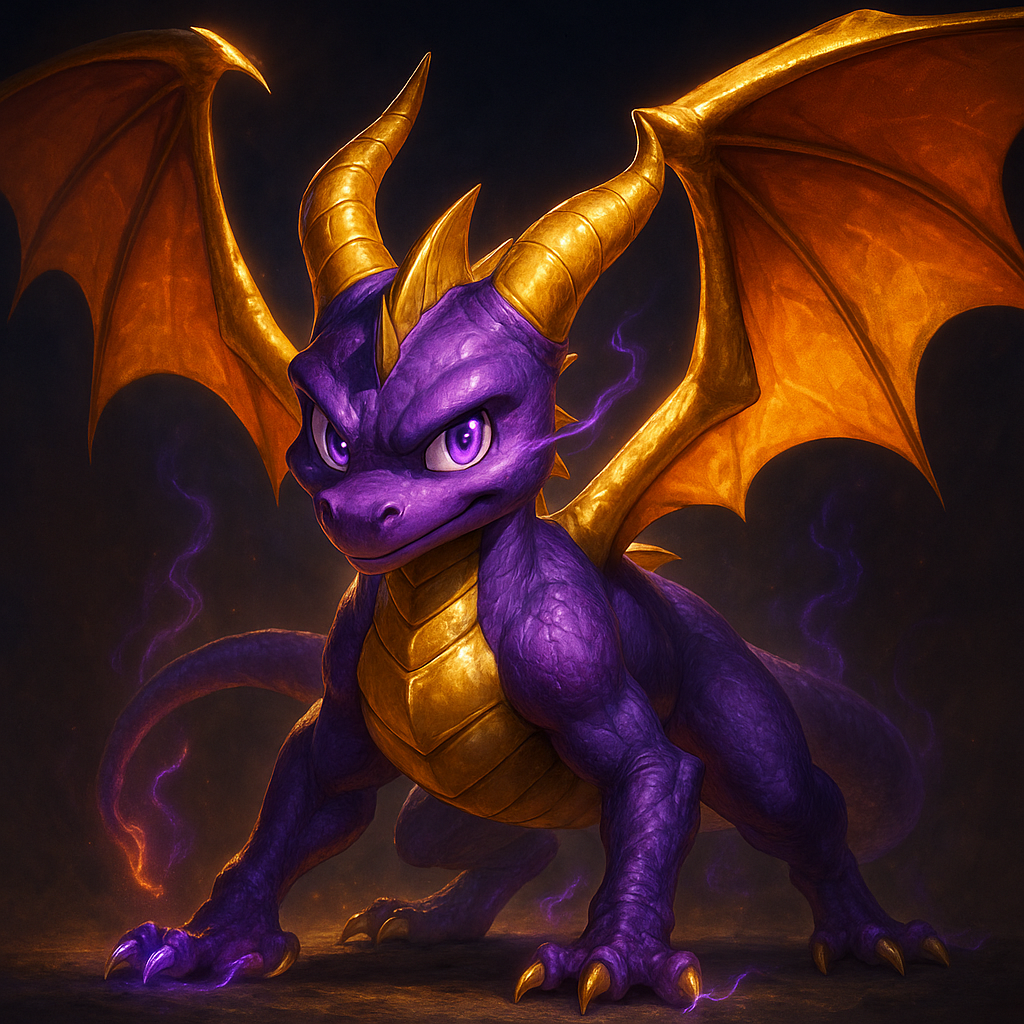
\includegraphics[width=0.5\textwidth]{example-image.png}
\caption{An example image}
\end{figure}
\lipsum[9-16]
\end{lstlisting}

\begin{figure}[!htbp]
    \centering
    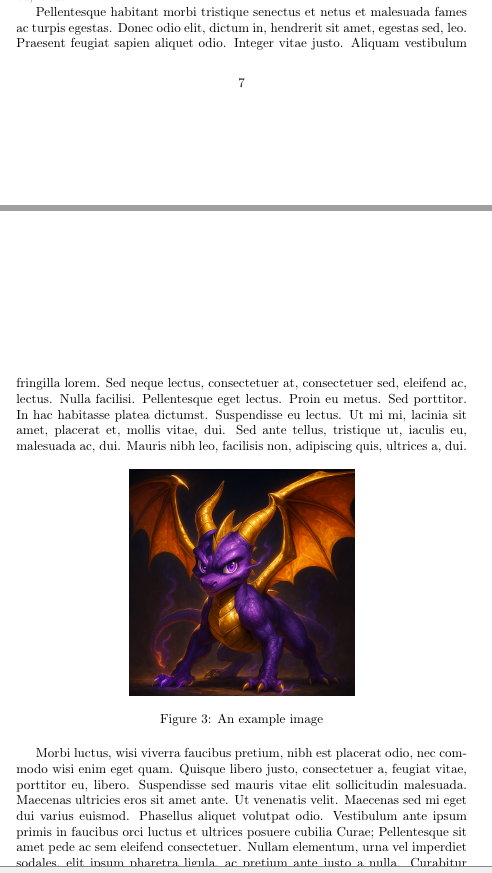
\includegraphics[width=0.8\textwidth]{image/5.png}
    \caption{Рисунок, зафиксированный в тексте с помощью опции [H]}
    \label{fig:005}
\end{figure}

\paragraph{1.6. Создание новых типов плавающих окружений.}
Пакет \texttt{trivfloat} позволяет создавать новые типы плавающих объектов. В примере был создан новый тип \texttt{image}. Код показан в \lstlistingname~\ref{lst:part1_6}, результат --- на \figurename~\ref{fig:006}.

\begin{lstlisting}[
    float=htbp,
    language=tex,
    caption={Новый тип плавающего окружения с trivfloat},
    label=lst:part1_6
]
\usepackage{trivfloat}
\trivfloat{image}
...
trivfloat image
\begin{image}
\centering
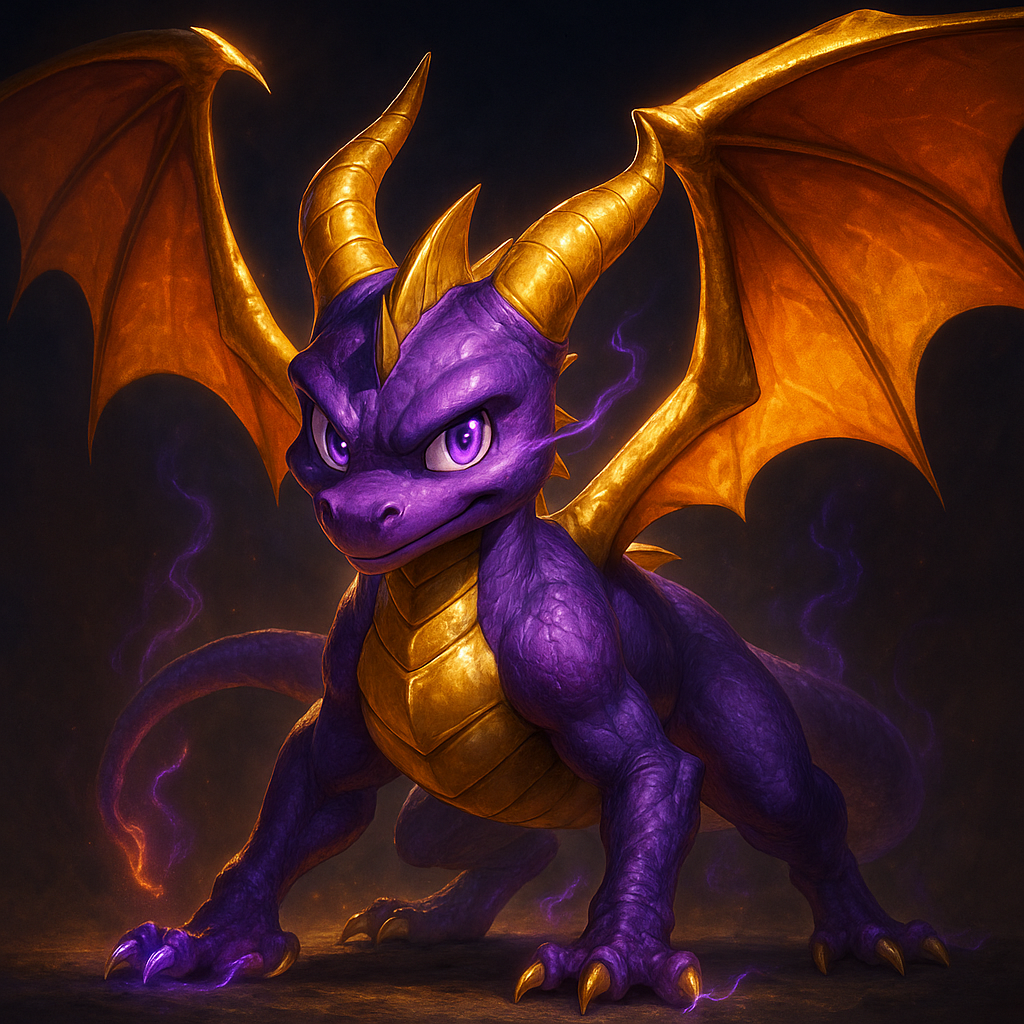
\includegraphics[width=0.5\textwidth]{example-image.png}
\caption{An example image}
\end{image}
\end{lstlisting}

\begin{figure}[!htbp]
    \centering
    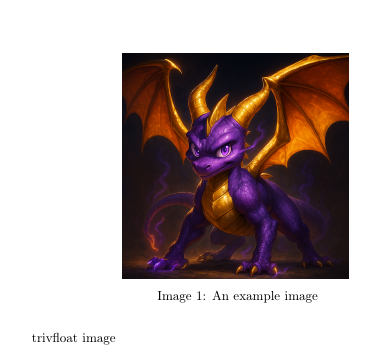
\includegraphics[width=0.8\textwidth]{image/6.png}
    \caption{Результат использования окружения `image` из `trivfloat`}
    \label{fig:006}
\end{figure}

\paragraph{1.7. Создание перекрёстных ссылок.}
Была реализована система ссылок на раздел и уравнение с помощью команд \texttt{\textbackslash label} и \texttt{\textbackslash ref}. Особое внимание было уделено неразрывному пробелу \texttt{\textasciitilde}, который предотвращает перенос строки между названием объекта (например, "уравнение") и его номером. Для корректного отображения потребовалось две компиляции. Код --- в \lstlistingname~\ref{lst:part1_7}, результат --- на \figurename~\ref{fig:007}.

\begin{lstlisting}[
    float=htbp,
    language=tex,
    caption={Перекрёстные ссылки на раздел и уравнение},
    label=lst:part1_7
]
\section{Title of the first section}
Hey world!

This is a first document.

\section{Title of the first section}

Text of material for the first section.

\subsection{Subsection of the first section}
\label{subsec:labelone}

Text of material for the first subsection.
\begin{equation}
e^{i\pi}+1 = 0
\label{eq:labeltwo}
\end{equation}

In subsection~\ref{subsec:labelone} is equation~\ref{eq:labeltwo}.
\end{lstlisting}

\begin{figure}[!htbp]
    \centering
    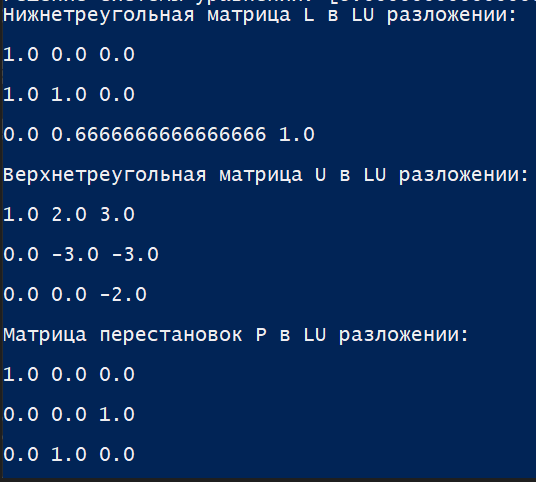
\includegraphics[width=0.8\textwidth]{image/7.png}
    \caption{Корректно отображённые перекрёстные ссылки}
    \label{fig:007}
\end{figure}

\paragraph{1.8. Кликабельные ссылки с hyperref.}
Для создания интерактивных ссылок в PDF-документе был подключен пакет \texttt{hyperref} с опцией \texttt{hidelinks} (но после оставлено без данной опции), чтобы убрать стандартную цветную рамку вокруг ссылок. Код --- в \lstlistingname~\ref{lst:part1_8}, результат --- на \figurename~\ref{fig:008}.

\begin{lstlisting}[
    float=htbp,
    language=tex,
    caption={Использование пакета hyperref},
    label=lst:part1_8
]
\usepackage[hidelinks]{hyperref}
...
\section{Introduction}

Some exciting text with a reference~\ref{sec:next}.

\section{Next thing}
\label{sec:next}

More text here. \lipsum[1]
\end{lstlisting}

\begin{figure}[!htbp]
    \centering
    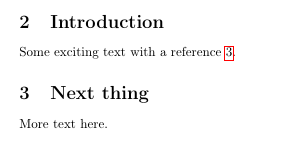
\includegraphics[width=0.8\textwidth]{image/8.png}
    \caption{Кликабельная ссылка в PDF-документе}
    \label{fig:008}
\end{figure}


\subsection{Часть 2: Выполнение упражнений}

\paragraph{2.1. Исследование опций \texttt{\textbackslash includegraphics}.}
Был вставлен собственный рисунок, и к нему были применены различные опции: \texttt{width}, \texttt{height}, \texttt{scale} (масштаб) и \texttt{angle} (поворот). Это позволило наглядно увидеть их влияние на итоговое изображение. Код --- в \lstlistingname~\ref{lst:part2_1}, результат --- на \figurename~\ref{fig:009}.

\begin{lstlisting}[
    float=htbp,
    language=tex,
    caption={Эксперименты с опциями \texttt{\textbackslash includegraphics}},
    label=lst:part2_1
]
Using different image options at Fig.~\ref{fig:my_image}.
\begin{figure}[H]
    \centering
    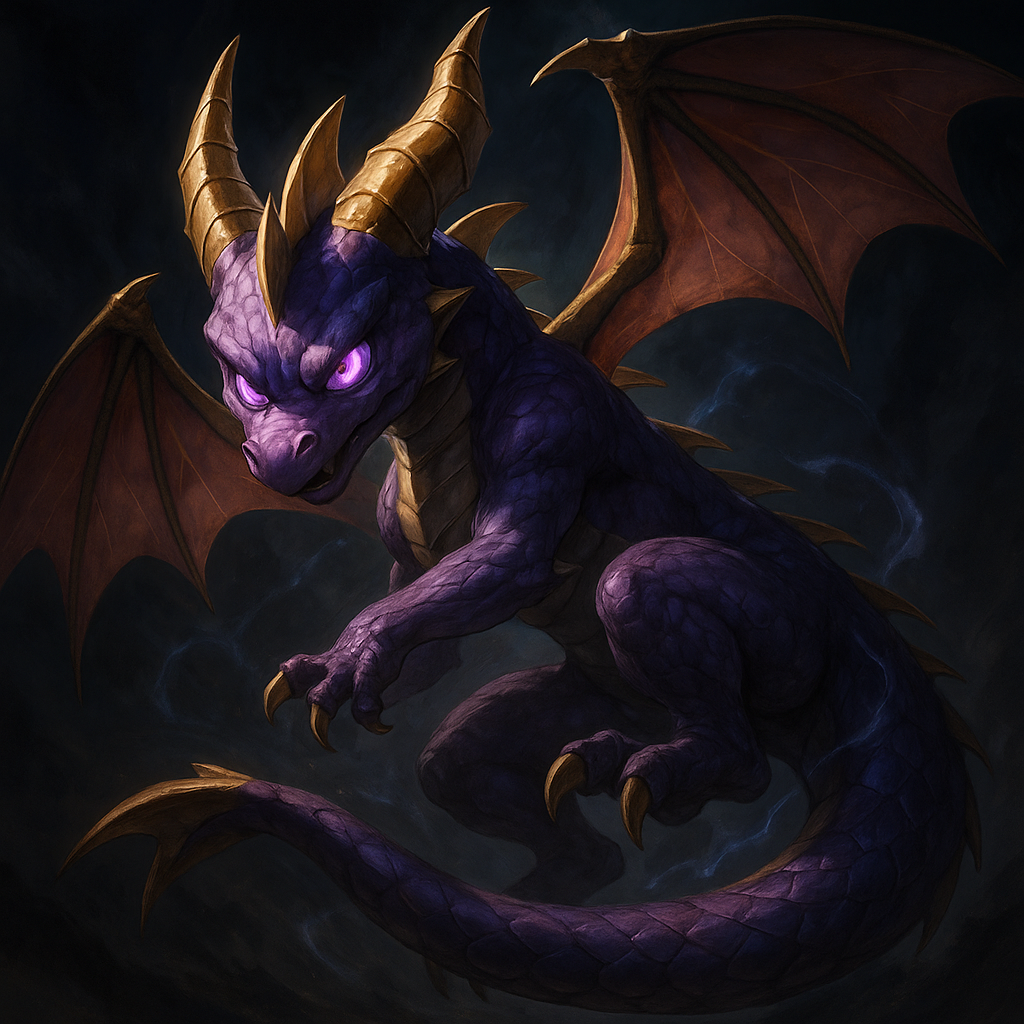
\includegraphics[width=0.7\textwidth,
                     height=4cm,
                     scale=0.8,
                     angle=15]
                     {example-image_b.png}
    \caption{Application of the options width, height, scale and angle}
    \label{fig:my_image}
\end{figure}
\end{lstlisting}

\begin{figure}[!htbp]
    \centering
    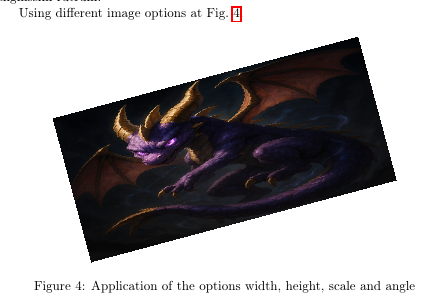
\includegraphics[width=0.8\textwidth]{image/9.png}
    \caption{Результат применения различных опций к изображению}
    \label{fig:009}
\end{figure}


\paragraph{2.2. Сравнение \texttt{\textbackslash textwidth} и \texttt{\textbackslash linewidth}.}
Для анализа разницы между \texttt{\textbackslash textwidth} и \texttt{\textbackslash linewidth} был создан документ в двухколоночном режиме (\texttt{twocolumn}).

Заметим, что \texttt{\textbackslash textwidth} --- это полная ширина текстового блока на странице, в то время как \texttt{\textbackslash linewidth} --- это ширина текущей строки. В двухколоночном режиме \texttt{\textbackslash linewidth} равна ширине одной колонки, а \texttt{\textbackslash textwidth} остаётся равной ширине обеих колонок вместе с промежутком. В результате изображение, масштабированное по \texttt{\textbackslash textwidth}, выходит далеко за пределы колонки, а по \texttt{\textbackslash linewidth} --- идеально вписывается в неё. Код --- в \lstlistingname~\ref{lst:part2_2}, результат --- на \figurename~\ref{fig:010}.

\begin{lstlisting}[
    float=htbp,
    language=tex,
    caption={Сравнение \texttt{\textbackslash textwidth} и \texttt{\textbackslash linewidth}},
    label=lst:part2_2
]
\documentclass[twocolumn]{article}
\usepackage{graphicx}
\usepackage{lipsum}
\begin{document}
\lipsum[1]

Width relative to \texttt{\textbackslash textwidth}:
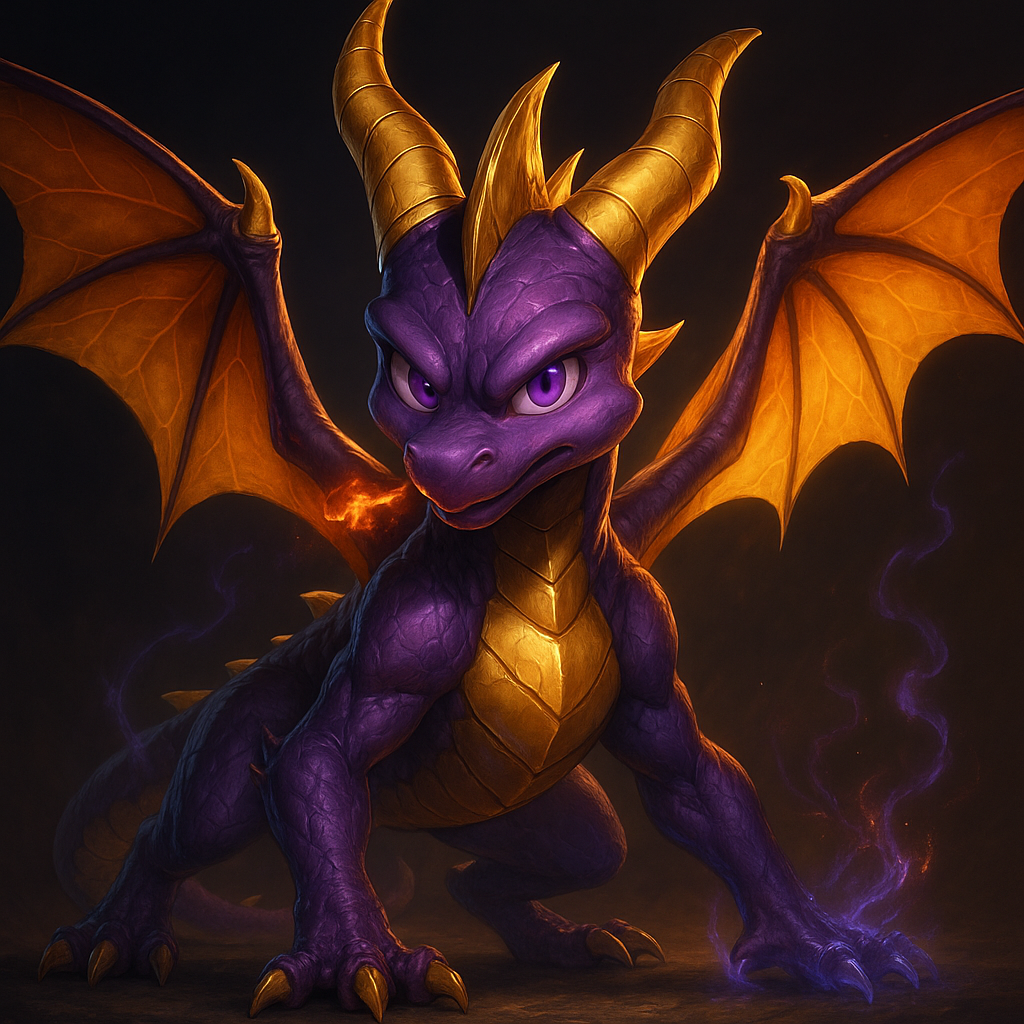
\includegraphics[width=0.6\textwidth]{example-image-a.png}

Width relative to \texttt{\textbackslash linewidth}:
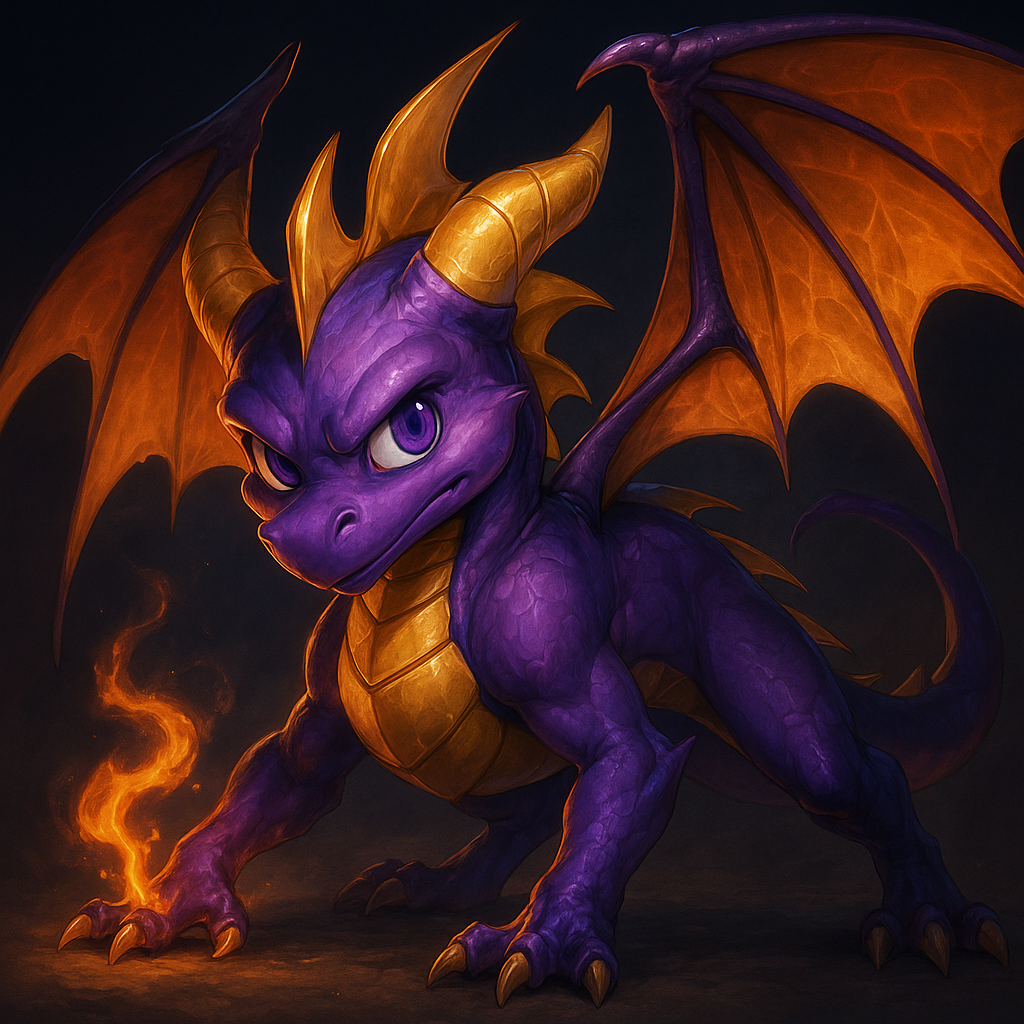
\includegraphics[width=0.8\linewidth]{example-image-c.png}

\lipsum[2-5]
\end{document}
\end{lstlisting}

\begin{figure}[!htbp]
    \centering
    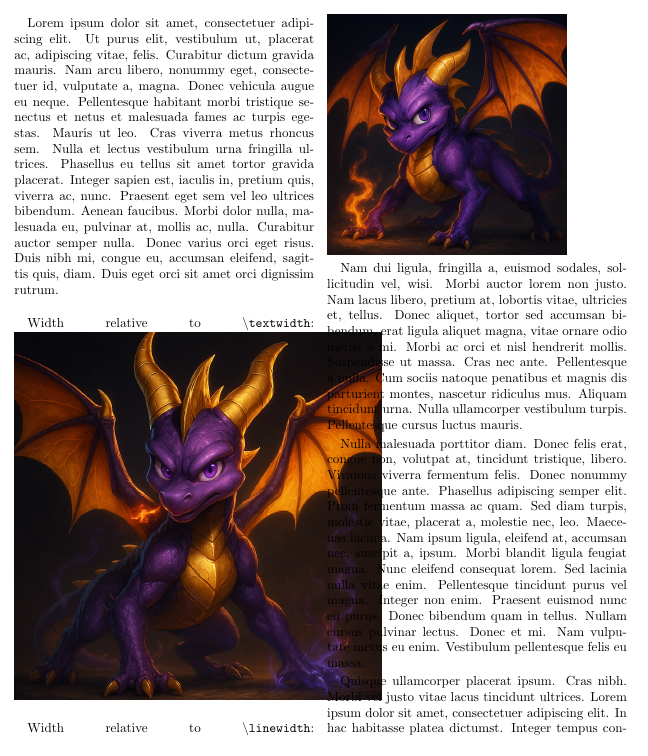
\includegraphics[width=0.8\textwidth]{image/10.png}
    \caption{Разница в поведении \texttt{\textbackslash textwidth} и \texttt{\textbackslash linewidth} в двухколончатом режиме}
    \label{fig:010}
\end{figure}

\paragraph{2.3. Эксперименты со спецификаторами размещения.}
Был создан длинный текст с плавающим рисунком, у которого менялись спецификаторы размещения (\texttt{[h]}, \texttt{[t]}, \texttt{[b]}, \texttt{[p]}, \texttt{[!htbp]}).

Спецификаторы работают как рекомендации для \LaTeX.
\begin{itemize}
    \item \texttt{h} (here): пытается разместить объект здесь. Работает только если есть место.
    \item \texttt{t} (top): разрешает размещение вверху страницы.
    \item \texttt{b} (bottom): разрешает размещение внизу страницы.
    \item \texttt{p} (page): разрешает вынос на отдельную страницу с плавающими объектами.
\end{itemize}
Комбинация \texttt{[!htbp]} даёт \LaTeX максимальную свободу и обычно приводит к наилучшему результату с точки зрения типографики. Код --- в \lstlistingname~\ref{lst:part2_3}, результат --- на \figurename~\ref{fig:011}.

\begin{lstlisting}[
    float=htbp,
    language=tex,
    caption={Сравнение расположений изображения с различными спецификаторами},
    label=lst:part2_3
]
\lipsum[1-3]
\begin{figure}[!htbp]
\centering
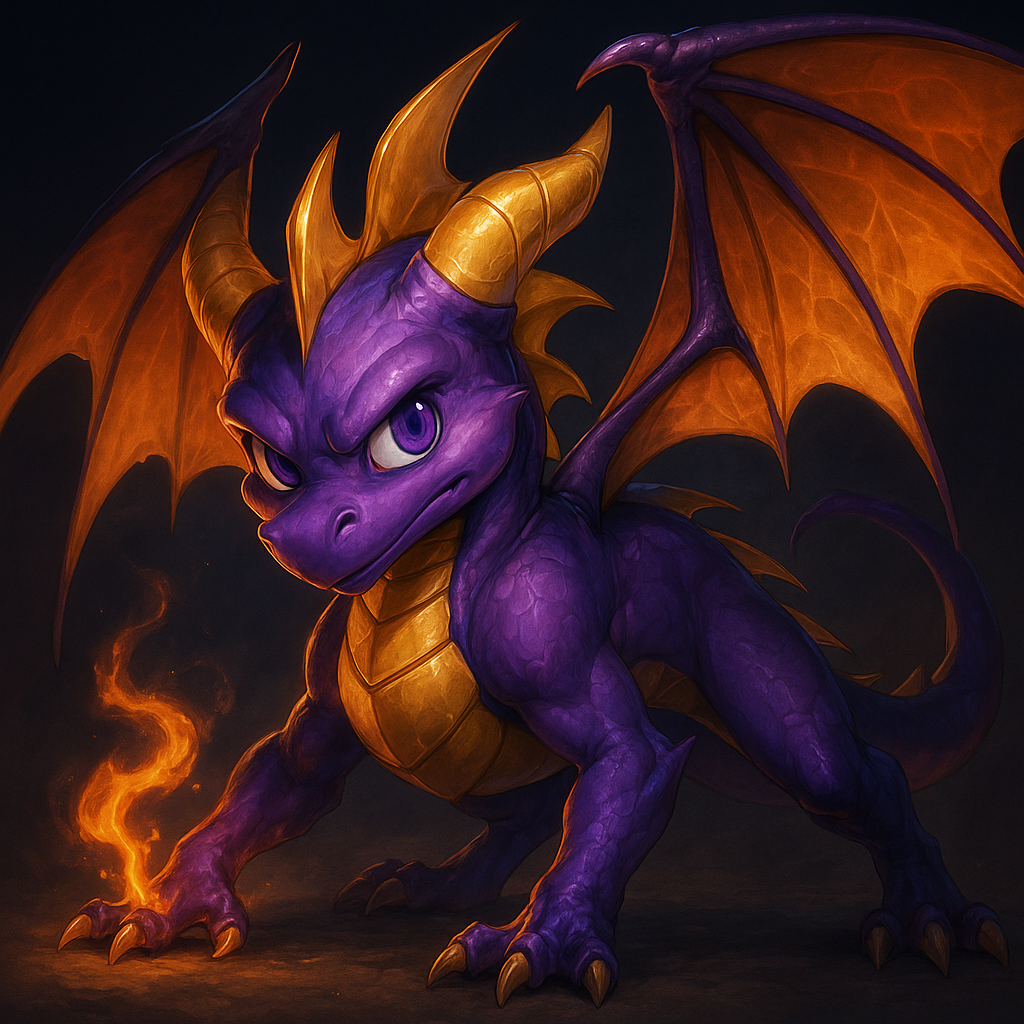
\includegraphics[width=0.5\textwidth]{example-image-c.png}
\caption{An example image}
\end{figure}
\lipsum[4-5]
\end{lstlisting}

\begin{figure}[!htbp]
    \centering
    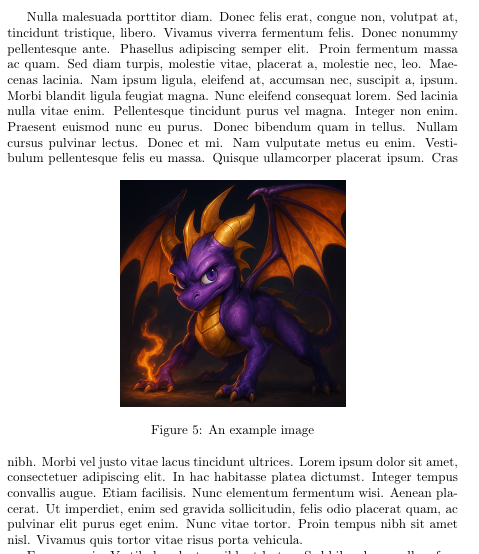
\includegraphics[width=0.8\textwidth]{image/11.png}
    \caption{Наилучший результат расположения изображения со спецификатором \texttt{[!htbp]}}
    \label{fig:011}
\end{figure}

\paragraph{2.4. Стабилизация ссылок.}
В документ были добавлены новые нумерованные элементы (подраздел и список \texttt{enumerate}) и установлены на них ссылки. 

При первой компиляции \LaTeX видит метки \texttt{\textbackslash label}, но ещё не знает их значений. Он записывает их в \texttt{.aux} файл. Ссылки \texttt{\textbackslash ref} отображаются как \texttt{??}. При второй компиляции \LaTeX читает \texttt{.aux} файл и подставляет правильные номера. Если структура документа сложная, может потребоваться и третья компиляция. В данном случае \textbf{стабилизация всех ссылок произошла за 2 прогона компилятора}. При этом ссылка на нумерованный список как результат отметила номер подраздела. Код --- в \lstlistingname~\ref{lst:part2_4}, Результат на \figurename~\ref{fig:012}.

\begin{lstlisting}[
    float=htbp,
    language=tex,
    caption={Добавление новых ссылок на раздел, подраздел, нумерованный список},
    label=lst:part2_4
]
\section{Label Test}
\label{sec:labtest}

Text of the section~\ref{sec:labtest} for label testing.

\subsection{Enumerate label test}
\label{subsec:enlabtest}

Here in subsection~\ref{subsec:enlabtest} we test enumerate list and it's label~\ref{en:test}
\begin{enumerate}
\label{en:test}
\item \lipsum[1]
\item \lipsum[2]
\end{enumerate}
\end{lstlisting}

\begin{figure}[!htbp]
    \centering
    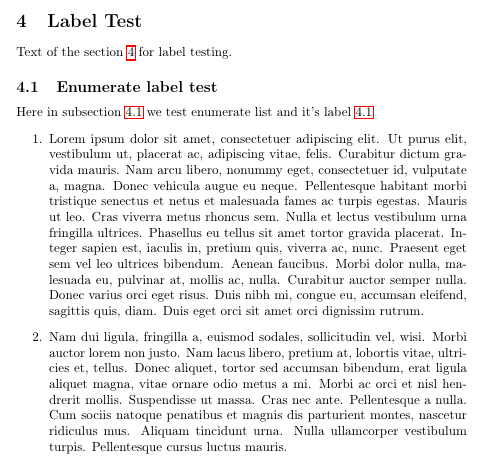
\includegraphics[width=0.8\textwidth]{image/12.png}
    \caption{Ссылки на новые элементы: подраздел и пункт списка}
    \label{fig:012}
\end{figure}

\paragraph{2.5. Важность порядка команд \texttt{\textbackslash label} и \texttt{\textbackslash caption}.}
Команда \texttt{\textbackslash label} была помещена \textit{до} команды \texttt{\textbackslash caption} внутри окружения \texttt{figure}.

Команда \texttt{\textbackslash label} всегда ссылается на последний инкрементированный счётчик, а команда \texttt{\textbackslash caption} как раз и отвечает за увеличение счётчика рисунков (\texttt{figure}). Если \texttt{\textbackslash label} стоит до неё, то она находит предыдущий счётчик, которым в данном случае был счётчик подразделов (\texttt{subsection}). В итоге, ссылка \texttt{\textbackslash ref} указывает не на номер рисунка, а на номер подраздела. Таким образом, команду \texttt{\textbackslash label} для плавающих объектов необходимо всегда ставить \textbf{после} команды \texttt{\textbackslash caption}. Код --- в \lstlistingname~\ref{lst:part2_5}, Результат эксперимента на \figurename~\ref{fig:013}.

\begin{lstlisting}[
    float=htbp,
    language=tex,
    caption={Неправильный порядок \texttt{\textbackslash label} и \texttt{\textbackslash caption}},
    label=lst:part2_5
]
Then we test wrong label to an image with a caption.
\begin{figure}[H]
    \centering
    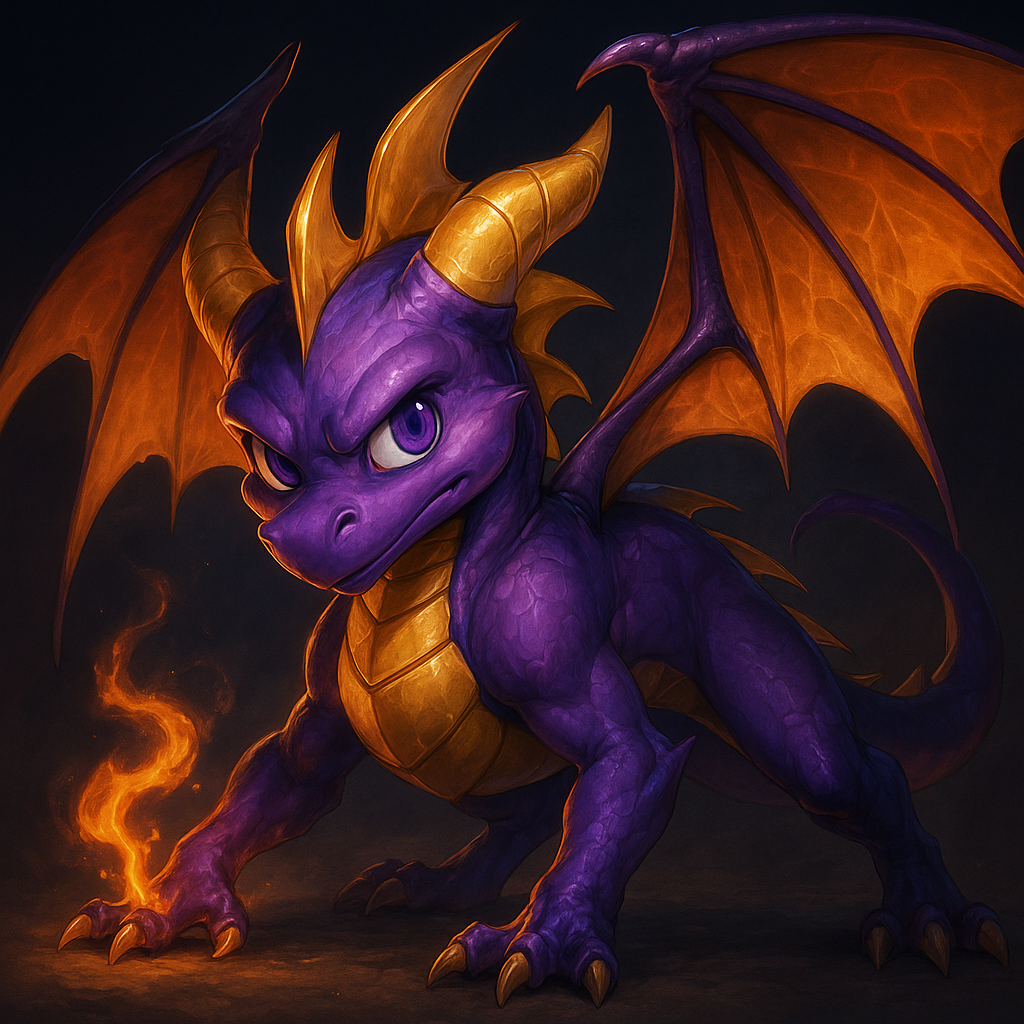
\includegraphics[width=0.3\textwidth]{example-image-c.png}
    \label{fig:wrong_label_order} % Неправильно!
    \caption{A figure with incorrect label order.}
\end{figure}
A reference to figure~\ref{fig:wrong_label_order}. % Ссылка будет на номер подраздела
\end{lstlisting}

\begin{figure}[!htbp]
    \centering
    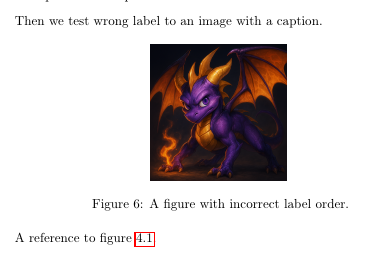
\includegraphics[width=0.8\textwidth]{image/13.png}
    \caption{Некорректная ссылка на изображение из-за неправильного порядка команд}
    \label{fig:013}
\end{figure}

\paragraph{2.6. \texttt{\textbackslash label} вне окружения \texttt{equation}.}
Команда \texttt{\textbackslash label} была помещена \textit{после} \texttt{\textbackslash end\{equation\}}.

Это аналогично предыдущему пункту. Окружение \texttt{equation} --- это область, где создаётся и нумеруется формула. Как только \LaTeX встречает \texttt{\textbackslash end\{equation\}}, счётчик формул перестаёт быть активным. Команда \texttt{\textbackslash label}, расположенная снаружи, снова находит счётчик подраздела. Ссылка не сработает, как ожидалось, а значит, команда \texttt{\textbackslash label} для нумерованного объекта должна находиться внутри его окружения. Код --- в \lstlistingname~\ref{lst:part2_6}, Результат эксперимента на \figurename~\ref{fig:014}.

\begin{lstlisting}[
    float=htbp,
    language=tex,
    caption={Неправильный порядок \texttt{\textbackslash label} и \texttt{\textbackslash end\{equation\}}},
    label=lst:part2_6
]
\subsection{Equation label test}
\label{subsec:eqlabtest}

And finally, here in subsection~\ref{subsec:eqlabtest} we test wrong label for an equation~\ref{eq:test}
\begin{equation}
e = mc^2
\end{equation}
\label{eq:test} 
\end{lstlisting}

\begin{figure}[!htbp]
    \centering
    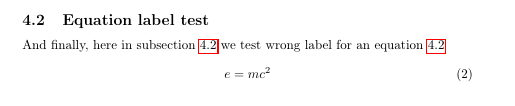
\includegraphics[width=0.8\textwidth]{image/14.png}
    \caption{Некорректная ссылка на уравнение из-за неправильного порядка команд}
    \label{fig:014}
\end{figure}

\section{Выводы}
В ходе выполнения данной лабораторной работы я получил практические навыки по работе с графикой и системой перекрёстных ссылок в \LaTeX. Были освоены:
\begin{itemize}
    \item Вставка и настройка изображений с помощью пакета \texttt{graphicx}, включая масштабирование, кадрирование и поворот.
    \item Управление расположением графики с помощью плавающих окружений (\texttt{figure}) и средств их "жёсткой" фиксации (пакет \texttt{float}).
    \item Организация структуры проекта с выносом изображений в подкаталоги (\texttt{\textbackslash graphicspath}).
    \item Создание системы перекрёстных ссылок на разделы, рисунки, уравнения и другие элементы с помощью команд \texttt{\textbackslash label} и \texttt{\textbackslash ref}.
    \item Понимание важности порядка команд (\texttt{\textbackslash caption} перед \texttt{\textbackslash label}) и области видимости меток.
    \item Улучшение интерактивности итогового документа за счёт кликабельных ссылок, предоставляемых пакетом \texttt{hyperref}.
\end{itemize}

\printbibliography
  
\end{document}